\documentclass[UTF8]{ctexart}
\usepackage{subfiles}  

%下面的语句, 引入你的头部设置文件
\usepackage{C:/phpStorm_proj/02_myself_ID_EGO/+100_latex_all_math_sel/myPreamble} 
%必须是绝对路径,才能让各个tex在单独编译时使用到

\title{向量组的 秩}


%---------------------------------


\begin{document}
\tableofcontents % 生成目录
\date{} % 若不写这句, 则默认也会渲染出日期, 所以我们要手动赋空值
\maketitle  %这行代码, 让你前面的 title, author, date生效

\section{极大线性无关组}

极大线性无关组 maximal linearly independent system: 就是在线性空间中, 拥有向量个数最多的那一个``线性无关的向量组". 其实就是在一个向量组, 最多有几个``基轴"的概念.  \\

比如, 有一个向量组A: $\alpha_1, ..., \alpha_5$, 其中:\\
- $\alpha_1, \alpha_2$ 是线性无关的, 即它们就属于基轴了. \\
- 这个向量组A中的每一个向量, 都可由基轴$\alpha_1, \alpha_2$来表示. \\
则, $\alpha_1, \alpha_2$ 就称为是这个向量组A 的``极大线性无关组". \\

注意: 在一个向量组中, 找其子集``极大线性无关组", 可能是不唯一的(即基轴不唯一). \\ 

\begin{myEnvSample}
比如:  \\
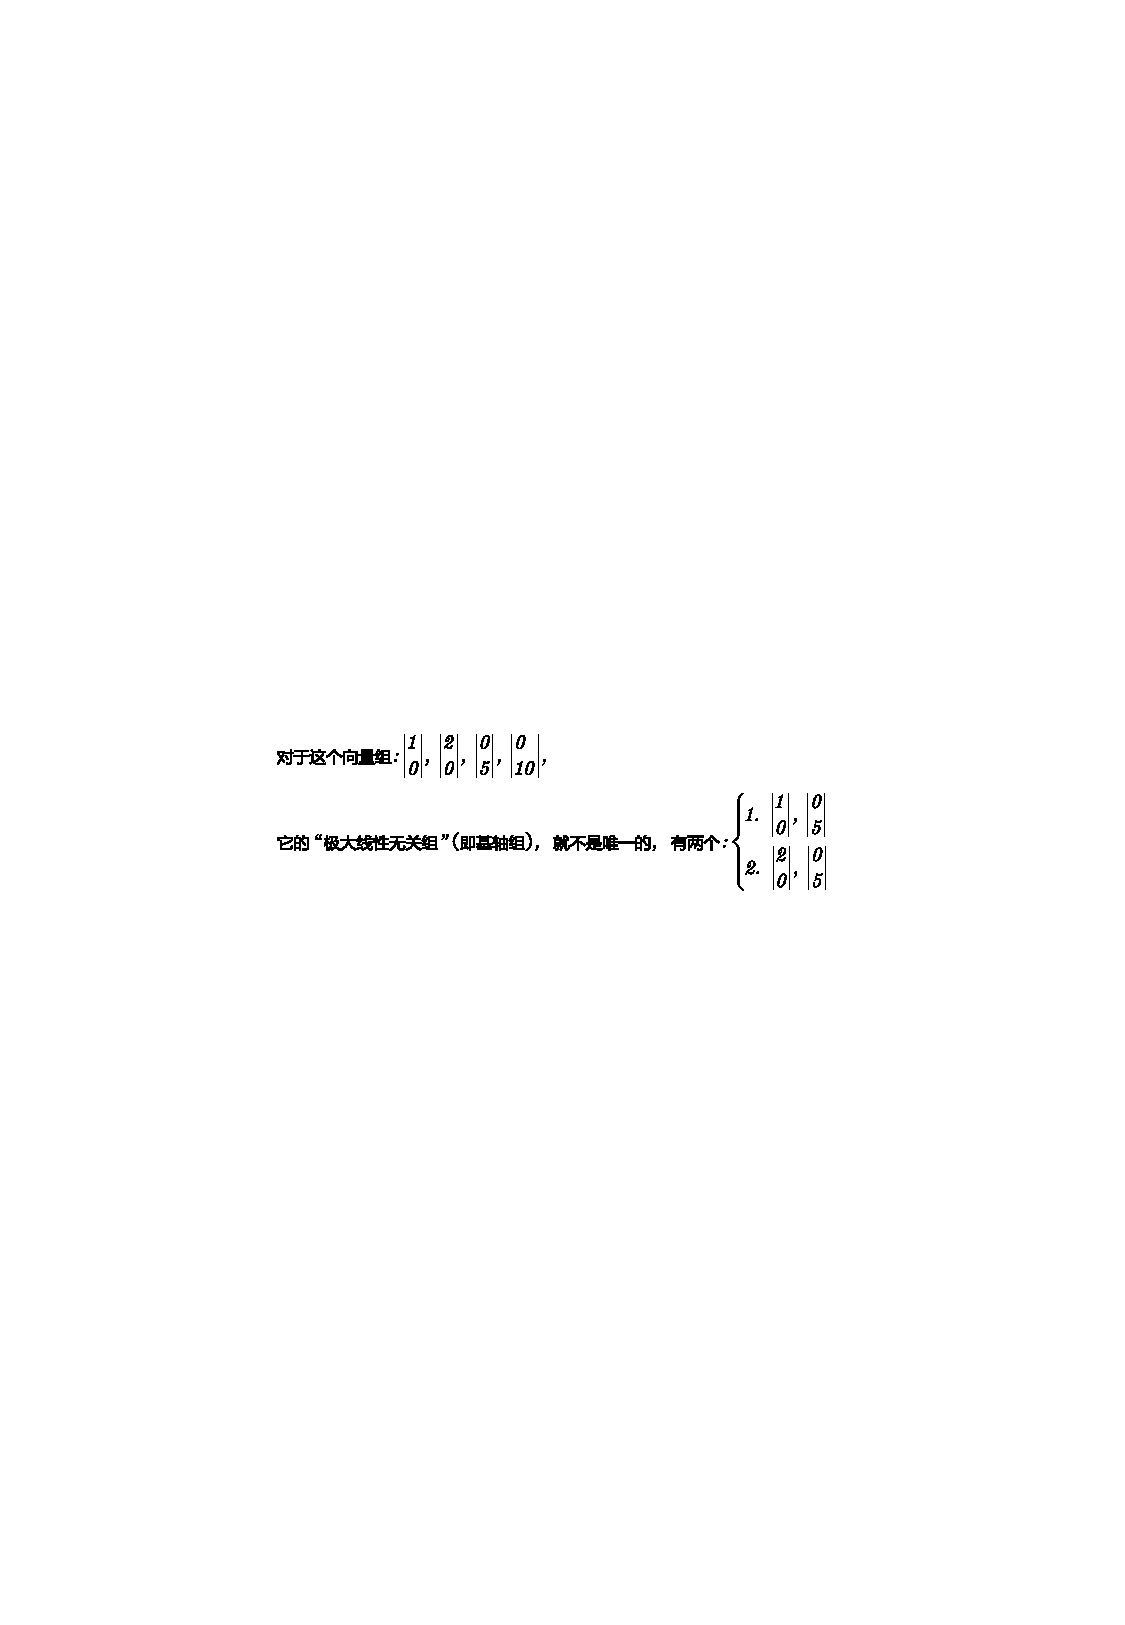
\includegraphics[width=0.8\textwidth]{img/0110.pdf}
\end{myEnvSample}


~\\
\hrule
~\\

\section{向量组的秩 rank: 就是该向量组的``极大线性无关组"中所含向量的个数}

注意: ``向量组的秩", 和``矩阵的秩", 定义并不相同. \\

一个向量组, 由$\alpha _1,...\alpha _s$这些向量构成, 则, 该向量组的秩, 数量范围就是在: 
\begin{align*}
0\leq \underset{\text{该向量组的}rank\text{数}}{\underbrace{r\left( \alpha _1,...\alpha _s \right) }}\leq \underset{\text{取两者中的最小者}}{\underbrace{\min\text{\{该向量组中的向量个数,向量的维度数\}}}}
\end{align*}

比如, 在3维空间中, 有10个3维的向量, 则, 该向量组的秩(基轴数), 就是3了.\\

所以, 我们就知道: \\
→ 如果一个向量组(含有s个向量)的秩数r = s 的话, 那么这个向量组中的向量, 就是``线性无关"的. 即每个向量都成为了一个基轴.\\
→ 如果一个向量组 $\alpha _1,...\alpha _s$中的向量, 是``线性相关"的, 则: 该向量组的秩数 r 就小于 s. \\

~\\
\hrule
~\\

\section{矩阵的行秩, 和列秩}

把一个矩阵的每一行, 拿出来, 作为``行向量组", 则这个``行向量组"的秩, 就叫``行秩". \\
把一个矩阵的每一列, 拿出来, 作为``列向量组", 则这个``列向量组"的秩, 就叫``列秩". \\

有定理: 

\subsection{矩阵的 行秩=列秩=矩阵的秩 r(A)}











% https://www.bilibili.com/video/BV1aW411Q7x1?p=25&vd_source=52c6cb2c1143f8e222795afbab2ab1b5




\end{document}